\documentclass[12pt]{article}
\usepackage{blubird}
% has options [nodate, nosans, nofancy, nocolor, code]

% TITLE
\title{Expositions}
\author{Bryan Lu}
\date{5 June 2023} % do not use if [nodate] option enabled

\begin{document}
\maketitle

The rest of this lecture will proceed in a ``choose your own adventure'' format:
For each of the first three \tbf{Core Ideas}, you will get to pick one of the
two stories to talk about via democracy. These are notes to follow 
for every possible branch the talk may take. 

\section{Connections}
\subsection{How to Tell Spaces Apart (Simplicial Homology)}
From a study of planar graphs or polyhedra, one might recall the \tbf{Euler
characteristic} -- for a graph $G$ with $V$ vertices, $E$ edges, and $F$ faces
(including the ``outside'' if necessary) we have $\chi(G) = V - E + F$. For
planar graphs and polyhedral graphs we know that $\chi(G)$ = 2. 

Let's do it with what will look like roughly the same graph on paper, but we'll
play around with gluing various edges together in various ways. 
\begin{exercise}
  Identify as many of the following shapes as you can. A correct answer will be
  ``continuously deformable'' into the pictures shown -- they don't have to be
  exact matches! Vertices of the same color should also be thought of as being
  ``glued together.'' 
\begin{center}
    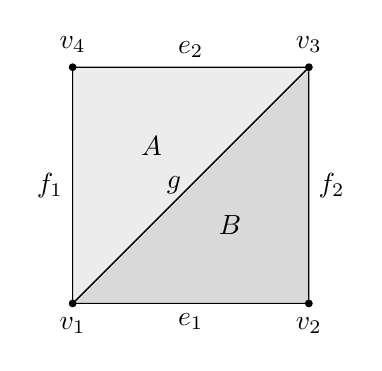
\begin{tikzpicture}
        \draw[fill=gray!30] (0,0) -- ++(3,0) -- ++(0, 3) -- ++(-3,-3) ;
       \node[circle,inner sep=1pt](D) at (2,1) {$B$};
       \draw[fill=gray!15] (0,0) -- ++(0,3) -- ++(3, 0) -- ++(-3,-3) ;
       \node[circle,inner sep=1pt](U) at (1,2) {$A$};
       \node[circle,fill,inner sep=1pt,label=below:$v_1$](p00) at (0,0) {};
       \node[circle,fill,inner sep=1pt,label=below:$v_2$](p10) at (3,0) {};
       \node[circle,fill,inner sep=1pt,label=above:$v_4$](p01) at (0,3) {};
       \node[circle,fill,inner sep=1pt,label=above:$v_3$](p11) at (3,3) {};

      \draw (p00) -- node[midway, above, left] {$g$} (p11);
      \draw (p00)  -- node[midway, below] {$e_1$} (p10) ;
      \draw (p01)  -- node[midway, above] {$e_2$} (p11) ;
      \draw (p00)  -- node[midway, left] {$f_1$} (p01) ;
      \draw (p10)  -- node[midway, right] {$f_2$} (p11) ;
    \end{tikzpicture}
    \begin{tikzpicture}
        \draw[fill=gray!30] (0,0) -- ++(3,0) -- ++(0, 3) -- ++(-3,-3) ;
       \node[circle,inner sep=1pt](D) at (2,1) {$B$};
       \draw[fill=gray!15] (0,0) -- ++(0,3) -- ++(3, 0) -- ++(-3,-3) ;
       \node[circle,inner sep=1pt](U) at (1,2) {$A$};
       \node[circle,fill,inner sep=1pt,label=below:$v_1$](p00) at (0,0) {};
       \node[circle,fill,inner sep=1pt,label=below:$v_2$](p10) at (3,0) {};
       \node[circle,fill,inner sep=1pt,label=above:$v_2$](p01) at (0,3) {};
       \node[circle,fill,inner sep=1pt,label=above:$v_3$](p11) at (3,3) {};

       \draw[-{Stealth[length=3mm, width=2mm]}, purple] (p00) -- node[midway, above, left] {$g$} (p11);
       \draw[-{Stealth[length=3mm, width=2mm]}, red] (p00)  -- node[midway, below] {$e$} (p10) ;
       \draw[-{Stealth[length=3mm, width=2mm]}, blue] (p01)  -- node[midway, above] {$f$} (p11) ;
       \draw[-{Stealth[length=3mm, width=2mm]}, red] (p00)  -- node[midway, left] {$e$} (p01) ;
       \draw[-{Stealth[length=3mm, width=2mm]}, blue] (p10)  -- node[midway, right] {$f$} (p11) ;
    \end{tikzpicture}
    \begin{tikzpicture}
        \draw[fill=gray!30] (0,0) -- ++(3,0) -- ++(0, 3) -- ++(-3,-3) ;
       \node[circle,inner sep=1pt](D) at (2,1) {$B$};
       \draw[fill=gray!15] (0,0) -- ++(0,3) -- ++(3, 0) -- ++(-3,-3) ;
       \node[circle,inner sep=1pt](U) at (1,2) {$A$};
       \node[circle,fill,inner sep=1pt,label=below:$v$](p00) at (0,0) {};
       \node[circle,fill,inner sep=1pt,label=below:$v$](p10) at (3,0) {};
       \node[circle,fill,inner sep=1pt,label=above:$v$](p01) at (0,3) {};
       \node[circle,fill,inner sep=1pt,label=above:$v$](p11) at (3,3) {};

       \draw[-{Stealth[length=3mm, width=2mm]}, purple] (p00) -- node[midway, above, left] {$g$} (p11);
       \draw[-{Stealth[length=3mm, width=2mm]}, red] (p00)  -- node[midway, below] {$e$} (p10) ;
       \draw[-{Stealth[length=3mm, width=2mm]}, red] (p01)  -- node[midway, above] {$e$} (p11) ;
       \draw[-{Stealth[length=3mm, width=2mm]}, blue] (p00)  -- node[midway, left] {$f$} (p01) ;
       \draw[-{Stealth[length=3mm, width=2mm]}, blue] (p10)  -- node[midway, right] {$f$} (p11) ;
    \end{tikzpicture}
\end{center}
\begin{center}
    \begin{tikzpicture}
        \draw[fill=gray!30] (0,0) -- ++(3,0) -- ++(0, 3) -- ++(-3,-3) ;
       \node[circle,inner sep=1pt](D) at (2,1) {$B$};
       \draw[fill=gray!15] (0,0) -- ++(0,3) -- ++(3, 0) -- ++(-3,-3) ;
       \node[circle,inner sep=1pt](U) at (1,2) {$A$};
       \node[circle,fill,inner sep=1pt,label=below:$v_2$](p00) at (0,0) {};
       \node[circle,fill,inner sep=1pt,label=below:$v_1$](p10) at (3,0) {};
       \node[circle,fill,inner sep=1pt,label=above:$v_1$](p01) at (0,3) {};
       \node[circle,fill,inner sep=1pt,label=above:$v_2$](p11) at (3,3) {};

      \draw[-{Stealth[length=3mm, width=2mm]}, purple] (p00) -- node[midway, above, left] {$g$} (p11);
      \draw[{Stealth[length=3mm, width=2mm]}-, red] (p00)  -- node[midway, below] {$e$} (p10) ;
      \draw[-{Stealth[length=3mm, width=2mm]}, red] (p01)  -- node[midway, above] {$e$} (p11) ;
      \draw[{Stealth[length=3mm, width=2mm]}-, blue] (p00)  -- node[midway, left] {$f$} (p01) ;
      \draw[-{Stealth[length=3mm, width=2mm]}, blue] (p10)  -- node[midway, right] {$f$} (p11) ;
    \end{tikzpicture}
    \begin{tikzpicture}
        \draw[fill=gray!30] (0,0) -- ++(3,0) -- ++(0, 3) -- ++(-3,-3) ;
       \node[circle,inner sep=1pt](D) at (2,1) {$B$};
       \draw[fill=gray!15] (0,0) -- ++(0,3) -- ++(3, 0) -- ++(-3,-3) ;
       \node[circle,inner sep=1pt](U) at (1,2) {$A$};
       \node[circle,fill,inner sep=1pt,label=below:$v$](p00) at (0,0) {};
       \node[circle,fill,inner sep=1pt,label=below:$v$](p10) at (3,0) {};
       \node[circle,fill,inner sep=1pt,label=above:$v$](p01) at (0,3) {};
       \node[circle,fill,inner sep=1pt,label=above:$v$](p11) at (3,3) {};

      \draw[-{Stealth[length=3mm, width=2mm]}, purple] (p00) -- node[midway, above, left] {$g$} (p11);
      \draw[-{Stealth[length=3mm, width=2mm]}, red] (p00)  -- node[midway, below] {$e$} (p10) ;
      \draw[-{Stealth[length=3mm, width=2mm]}, red] (p01)  -- node[midway, above] {$e$} (p11) ;
      \draw[-{Stealth[length=3mm, width=2mm]}, blue] (p00)  -- node[midway, left] {$f$} (p01) ;
      \draw[{Stealth[length=3mm, width=2mm]}-, blue] (p10)  -- node[midway, right] {$f$} (p11) ;
    \end{tikzpicture}
  
\end{center}
\end{exercise}
\noindent Keep these in mind! They will be our ``prototypical examples'' going
forward. 

How do you argue that the spaces that these graphs represent are
\tit{not isomorphic} to the normal plane $\RR^2$? One way is with the
Euler characteristics of all of these graph representations: 
  \begin{center}
    \begin{tabular}{c|ccccc}
      $G$ & (A) & (B) & (C) & (D) & (E) \\ \hline
      shape & $[0,1]^2$ & $S^2$ & $\TT^2$ & $\RR P^2$ & $K$ \\
      $\chi(G)$ & 2 & 2 & 0 & 1 & 0
    \end{tabular}
  \end{center}
  Note that the Euler characteristic isn't quite enough to differentiate the
surfaces depicted above -- after all, we only have one number. Let's really use
the structure of the graph now to analyze these surfaces at each dimension. 

First, for every top-dimensional triangular (simplicial) face (here,
2-dimensional), let's order the vertices so that when we do our gluing, the
orientation of the edges that are glued are consistent with the ordering of the
vertices. As an example:
  \begin{center}
  
    \begin{tikzpicture}
        \draw[fill=gray!30] (0,0) -- ++(3,0) -- ++(0, 3) -- ++(-3,-3) ;
       \node[circle,inner sep=1pt](D) at (2,1) {$B$};
       \draw[fill=gray!15] (0,0) -- ++(0,3) -- ++(3, 0) -- ++(-3,-3) ;
       \node[circle,inner sep=1pt](U) at (1,2) {$A$};
       \node[circle,fill,inner sep=1pt,label=below:$v \, (0 / 0)$](p00) at (0,0) {};
       \node[circle,fill,inner sep=1pt,label=below:$v \, (1)$](p10) at (3,0) {};
       \node[circle,fill,inner sep=1pt,label=above:$v \, (1)$](p01) at (0,3) {};
       \node[circle,fill,inner sep=1pt,label=above:$v \, (2 / 2)$](p11) at (3,3) {};

      \draw[-{Stealth[length=3mm, width=2mm]}, purple] (p00) -- node[midway, above, left] {$g$} (p11);
      \draw[-{Stealth[length=3mm, width=2mm]}, red] (p00)  -- node[midway, below] {$e$} (p10) ;
      \draw[-{Stealth[length=3mm, width=2mm]}, red] (p01)  -- node[midway, above] {$e$} (p11) ;
      \draw[-{Stealth[length=3mm, width=2mm]}, blue] (p00)  -- node[midway, left] {$f$} (p01) ;
      \draw[-{Stealth[length=3mm, width=2mm]}, blue] (p10)  -- node[midway, left] {$f$} (p11) ;
    \end{tikzpicture}
  \end{center}
In general, we might have an $n$-dimensional \tbf{simplex} as a part of our
space $G$, which we define as a continuous image of the canonical $n$-simplex
$\Delta^n = \set{\bf x \in \RR^{n+1} : \sum_{i=1}^{n+1} x_i = 1, x_i \geq
0}$ into $G$, which we also write in terms of its vertices $[v_0, v_1,
\dots, v_n]$. The relationship between dimensions is one of the
\tbf{boundary} -- for instance, when we take an $n$-dimensional simplex of our
space, its boundary is a union of $(n-1)$-simplices. With the orientation on each
simplex, we define the \tbf{boundary map} acting on an $n$-simplex $\sigma$ to be the
following formal sum of $n-1$-simplices: 
\[
\bound \sigma = \sum_{i=0}^n (-1)^i \sigma\big|_{[v_0, v_1, \dots, v_{i-1},
v_{i+1}, \dots, v_n]}
\]
The signs are maybe a surprising addition -- but with this, one can consider the
integer linear combinations of all of the $k$-dimensional simplices $C_k(G)$ for
one of our spaces, and the boundary maps assemble the $C_k$s into a \tbf{chain
complex}:
\[
  \dots \to C_n(G) \xto {\partial_n} \dots \to C_2(G) \xto{\partial_2} C_1(G)
  \xto{\partial_1} C_0(G) \xto{\partial_0} 0  
\]
where we extend the boundary maps to act linearly on integer linear combinations
of simplices. 

The key observation (due to Emmy N\"oether and Mayer/Vietoris) -- if the boundary of a suitable sum of simplices is 0,
these simplices encircle a closed region in $G$. But, if such a sum of
simplices is not the boundary of any simplex in $G$, then we have
detected a hole within our space! Therefore, the linear subspace of $C_n$
that encircles closed regions in $G$ but ignoring any parts of it that actually
do describe closed regions in $G$, gives us a subspace spanned by the
holes of $G$! Interpreting this from the lens of linear
algebra, we define the \tbf{homology groups} 
\[
\boxed{H_n(G) = \frac{\ker \bound_n}{\im \bound_{n+1}}} 
\] 
As a fact to make these well-defined, we need to know that $\boxed{\bound^2 = 0}$, which
is a defining feature of a general chain complex (that I've omitted until now).   
Now we can basically use linear algebra to compute them, since a basis of
these subspaces tells us exactly where the holes are in our space at any
dimension we like! This is the construct that will allow us to make more
granular comparisons between spaces:  
\begin{center}
    \begin{tabular}{c|ccccc}
      $G$ & $S^2$ & $\TT^2$ & $\RR P^2$ & $K$ \\ \hline
      $H_0(G)$ & $\ZZ$ & $\ZZ$ & $\ZZ$ & $\ZZ$ \\ 
      $H_1(G)$ & $0$ & $\ZZ^2$ & $\ZZ / 2 \ZZ $ & $\ZZ \times \ZZ / 2\ZZ$ \\ 
      $H_2(G)$ & $\ZZ$ & $\ZZ$ & $0$ & $0$ \\ 
    \end{tabular}
\end{center}
\begin{exercise}
We can also recover the Euler characteristic from these groups! For a general
topological space, the Euler characteristic is defined as $\chi(G) =
\sum_{i=0}^\infty (-1)^i \dim_{\ZZ} H_i(G)$ (where the dimension here ignores
any non-$\ZZ$ factors in the homology). Check this!  
\end{exercise}

This construct isn't a panacea -- there are spaces that homology cannot tell
apart. For instance, consider the space constructed by gluing a sphere and two
circles together all at the same point. The homology of a torus/doughnut is
identical to this! Other tools have to come into play to tell these spaces
apart (cohomology, homotopy). However, homology is still very powerful!    
\begin{idea}
  Representing general (topological) spaces as graphs is very
powerful and fairly general, and allows one to study them with algebraic tools.
\end{idea}


\subsection{Word Problems (Geometric Group Theory)}
Let's talk about \tbf{groups}! Formally, a group is a set $G$ with a binary
operation $m : G \times G \to G$ and inverses with respect to $m$, given by $i :
G \to G$ such that $m$ is associative and has an identity such that multiplying
any element by its inverse gives the identity. Let's take a more constructive
approach instead though: 

\begin{definition*}
  Suppose $S$ is a set of symbols, and let $S^{-1}$ be the collection of formal
  symbols consisting of $\set{s^{-1} : s \in S}$. Let $R$ be a collection of
  (non-empty) strings in $S$ or $S^{-1}$, i.e. $R \subseteq L(S \cup S^{-1})$.
  Two words $u, v \in L(S \cup S^{-1})$ are \tit{equivalent} (giving an
  equivalence relation $\sim$) if there is a
  sequence of moves turning $u$ into $v$ such that each move either adds or
  removes a pair $s s^{-1}$ or $s^{-1} s$ for $s \in S$, or adds or removes
  some $r \in R$. 
\end{definition*}
\begin{definition*}
  The collection of equivalence classes of $L(S \cup S^{-1}) /
  \sim$, where $\sim$ is generated by $S$ and $R \subseteq L(S \cup S^{-1}$), is the group $G$ with \tbf{presentation} $\tuple{S \mid R}$ under
  concatenation and reversals/inversions. $S$ is said to be the set of
  \tbf{generators} of $G$, and $R$ is the set of \tbf{relations}.  
\end{definition*}
\begin{exercise}
  Identify as many of the following groups from their presentations as you can: 
\begin{center}
  \begin{multicols}{3}
    \begin{enumerate}[label=(\alph*)]
    \item $\tuple{a \mid }$ 
    \item $\tuple{a \mid a^n}$ 
    \item $\tuple{a, b \mid a^3, b^2, (ab)^2 }$
    \item $\tuple{a, b \mid aba^{-1}b^{-1}}$ 
    \item $\tuple{a, b \mid a^n, b^2, (ab)^2 }$
    \item $\tuple{a, b \mid a^2, b^2}$
  \end{enumerate}
  \end{multicols}
\end{center}
\end{exercise}
We can use the presentation of a group to construct its \tbf{Cayley graph}: 
\begin{definition*}
  The \tbf{Cayley graph} of a group $G$ (not necessarily finite!) with generators $S$ 
  is a graph $\cay(G)$ with vertices $g$ for every $g \in G$ and directed edges
  from $g$ to $gs$ for every $g \in G$, $s \in S$.  
\end{definition*}
Be careful -- the directions of the edges do matter! We'll describe the
corresponding Cayley graphs for each of the above groups here:
\begin{multicols}{2}
\begin{enumerate}[label=(\alph*)]
  \item Directed line of vertices 
  \item Directed $n$-cycle
  \item Two triangles oriented in opposite directions, connected by edges between
    corresponding vertices
  \item 2D square lattice of edges going up and to the right
  \item Two $n$-gons oriented oppositely, connected by edges between
    corresponding vertices
  \item Undirected line of alternating-label edges 
\end{enumerate}  
\end{multicols}

\begin{remark}
One important application for Cayley graphs is that they are a natural space
for a \tbf{group action} of $G$. Essentially, this means there is a natural way
to ``multiply'' an element of the group $G$ and any element of the set, and for
the Cayley graph, we can simply consider left-multiplication by any group
element as the action.

One is often concerned with whether an action is \tbf{faithful} or \tbf{free},
which are slightly different measures of the ``injectivity'' of the action. An
action is faithful if there are no elements of the group that fix the entire set
other than the identity, and an action is free if for all non-identity elements
of the group, there are no fixed points of any of their actions. In particular,
the action of $G$ on its Cayley graph $\cay(G)$ is free. 
\end{remark}

We now introduce a problem that will drive the rest of this section:
\begin{problem}[The Word Problem]
  Given a group $G$ with finite presentation $\tuple{S \mid R}$ (i.e. $S$ and
  $R$ are both finite), for any word $w \in L(S \cup S^{-1})$, decide
  whether $[w]$ is the identity element $e$ in a finite amount of time.   
\end{problem}

While on the way to think about solving this problem for general groups, we can
study this problem in the Cayley graph of a group. Note that any word $w \in L(S
\cup S^{-1})$ represents a path in the Cayley graph starting at the identity
$e$, and a word that reduces to the identity is a loop at $e$, and vice versa.
As such, it suffices to check that the Cayley graph is \tbf{constructible} in a
finite amount of time -- this doesn't necessarily mean that we have to be able
to construct the entire Cayley graph, but instead that we should be able to
construct the subgraph of every vertex that is reachable in
at most $n$ steps from $e$ for arbitrarily large $n$. 

For the examples above, it's clear that we can do this quite easily by looking
at the Cayley graphs, and in fact many and most groups that we have a handle on
do have word problems can be solved. However, this problem still has a negative
answer in general: 
\begin{theorem}[Novikov-Boone]
  The word problem for finitely presented groups is \tbf{undecidable} -- in
  particular, there exists a finitely presented group $G$ for which the word
  problem is undecidable. 
\end{theorem}
And in fact, in connection to complexity theory, the following theorem
gives us a hint for how to construct such a group: 
\begin{theorem}[Higman's Embedding Theorem]
  Every finitely generated, \tbf{recursively presented} group $H$ can be embedded as a
 subgroup of some finitely presented group $G$, i.e. $H$'s
 set of relations is \tbf{recursively enumerable}. 
\end{theorem}
Roughly, recursive enumerability is less restrictive than decidability, as an 
algorithm/Turing machine only needs to terminate running on any element of the
set, not necessarily for all inputs. Using this theorem, we need only construct
a recursively presented group with undecidable word problem to break the word
problem in general!

\begin{remark}
One important class of examples are the \tbf{free groups} of rank $n$
  with $n$ generators and no relations, whose Cayley graphs are infinite trees
  with degree $2n$ at every vertex (with half of the generators going in/out of
  each vertex). As such, it's very easy to solve the word problem in these
  groups because there is a pretty easy algorithm to decide if we can reduce any
  word to the identity. 

  A surprising fact about free groups -- not only are they the only groups whose Cayley graphs
  are trees, they are the \tbf{only} groups that can act freely on trees! 
  This fact is important to showing that every subgroup of a free group is
  free (the \tbf{Nielson-Schreier} theorem), which is actually quite difficult
  to show otherwise.
\end{remark}

\begin{idea}
 Groups can be studied not only by their own structure, but also by their
 encodings as graphs and their actions on those graphs.   
\end{idea}

%\begin{itemize}
%  \item Galois theory and correspondences (examples in different contexts
%    too; covering spaces too?) 
%\subsubsection{Yet Another Galois Correspondence}
% this is too hard
%  \item Euler characteristic connecting to algebraic topology, simplicial homology
%
%  \item Lie algebra - group correspondence
% this is too hard 
%  \item solving the word problem 
%\end{itemize}

\noindent \tbf{(Enter break here, informal time for questions)}

\section{Generalizations}

\subsection{Doing Calculus Anywhere (Manifolds, Differential Forms)}
Many of you might recall the Fundamental Theorem of Calculus: 
\begin{theorem*}[Fundamental Theorem of Calculus]
  Let $f : U \to \RR$ be continuous on an open interval $U$ containing $[a, b]$,
  and $F : U \to \RR$ an antiderivative of $f$ on $(a, b)$, i.e. $F'(x) = f(x)$.
  Then \[
   \int_a^b f(x) \, dx = F(b) - F(a).
  \]  
\end{theorem*}
\noindent And some of you might recall the various ``fundamental theorems'' of
multivariable calculus:
\begin{center}
  \begin{minipage}{0.47\textwidth}
    \begin{theorem*}[Fund. Thm. of Line Integrals]
   Let $\vphi : U \to \RR$ be differentiable on an open subset $U \subseteq
   \RR^3$ and $\gamma : [0,1] \to U$ is a continuous curve in $U$.
   Then
   \[
    \int_\gamma \grad \vphi(\vect r) \cdot d\vect r = \vphi(\gamma(1)) -
    \vphi(\gamma(0)).
   \] 
  \end{theorem*} 
  \begin{theorem*}[Kelvin-Stokes Theorem]
    Let $\vect F : \RR^3 \to \RR^3$ be a $C^1$ vector field in an open region
    containing the smooth oriented surface $S$ in $\RR^3$, with boundary $\bound
    S$. 
    \[
      \iint_S (\curl \vect F) \cdot d\vect S = \oint_{\bound S} \vect F \cdot
      d\vect r
    \] 
  \end{theorem*}
  \end{minipage}
  \begin{minipage}{0.47\textwidth}
    \begin{theorem*}[Green's Theorem]
     Let $C$ be a positively oriented, simple rectifiable closed curve in
     $\RR^2$, bounding the region $D$. Let $L, M : \RR^2 \to \RR$ be $C^1$ on an
     open region containing $D$. Then
     \[
      \oint_C (L \, dx + M \, dy) = \iint_D \left( \pdv M x - \pdv L y \right)
      \, dx \, dy
     \] 
   \end{theorem*}
   \begin{theorem*}[Divergence Theorem]
     Let $V$ be a compact subset of $\RR^3$ with piecewise smooth boundary
     $\bound V$, and let $\vec F : \RR^3 \to \RR^3$ be a $C^1$ vector field. 
     Then
     \[
      \iint_V (\div \vect F) \, d V = \oiint_{\bound V} \vect F \cdot d \vect S
     \] 
   \end{theorem*}
  \end{minipage}
\end{center}
What are all of these theorems saying? They are all saying if one integrates a 
\tbf{function} over the \tbf{boundary of a space}, this is equal to 
integrating the \tbf{derivative} of that \tbf{function} over the entire \tbf{space}. 

How do we generalize this to arbitrary dimensions? Of course, we need a way to 
generalize ``space'', and likely also the notion of a derivative as it needs
to encompass gradient, divergence, and curl -- but what else? 
Looking at the proofs of these
theorems, especially Stokes' Theorem, might show us how to do it. Here is the
general sketch of the proofs for all of these theorems:
\begin{enumerate}
  \item Cut up the bounded region we are integrating over into little boxes,
    over which we perform the integration locally. 
  \item Doing an analysis on the interior of each box with the
    ``differentiated'' integrand, we show that this is equal to the
    ``undifferentiated'' integrand integrated over the boundary of the box.
    This step usually requires us to have some notion of the tangent
    vector/plane to the region at the point we are concerned at, and often to 
    combine this geometric information with the function being integrated  
  \item Piece the boxes back together, where the boundaries of the boxes in the
    interior cancel each other out.  
\end{enumerate}
This is, unsurprisingly, how the proof of the \tbf{generalized Stokes' Theorem}
goes, kind of, and the machinery that it entails does essentially this. 
Let's just state the general theorem and we'll break down what
everything is and why all of the above are just special cases of this. I've
color-coded all of the different components of this: 
\begin{theorem}[Generalized Stokes' Theorem]
  Let {\color{purple}$M$} be a $k$-dimensional \tbf{\color{blue} oriented} \tbf{\color{purple}
  smooth manifold-with-boundary} in $\RR^n$, and give the boundary
  {\color{purple}$\bound M$} the \tbf{\color{blue} boundary orientation}. Let
  {\color{orange}$\vphi$} be a smooth
  {\color{orange}$(k-1)$}\tbf{\color{orange}-form} defined on an open set
  containing $M$. Then 
  \[
    {\color{blue}\int_{\color{purple}\bound M} {\color{orange}\vphi}} =
    {\color{blue}\int_{\color{purple}
    M} {\color{red}\extd} {\color{orange}\vphi}}.
  \] 
\end{theorem}
\begin{proof}
  (Sketch.) Break up $M$ into parallelograms $P_i$ that in the limit, which 
  become vanishingly small, and also approximate the boundary $\bound M$. 
  Then $\int_M \extd\vphi = 
  \sum_i \extd\vphi = \sum_i \int_{\bound P_i} \vphi = \int_{\bound M} \vphi$, as desired. 
\end{proof}
\noindent Let's give a brief explanation for what (most of) everything is now: 
  
\noindent \tbf{\color{purple} What is a smooth manifold? What is its boundary?} A
    \tbf{manifold} in general can be defined in various ways. A traditional
    abstract definition might look like: 
    \begin{definition*}
      A $k$-dimensional smooth manifold $M$ is a topological space where every point $x \in M$ has a
      \tbf{chart} $\vphi_x : U_x \subseteq M \to V_x \subseteq \RR^k$ that are
      homeomorphisms (isomorphisms of topological spaces), such that the \tbf{transition
      maps} $\vphi_{x_2} \circ \vphi_{x_1}^{-1}$ are smooth maps from
      $V_{x_1} \subseteq \RR^k \to \RR^k$ if $U_{x_1} \cap U_{x_2}$ is non-empty.  
    \end{definition*}
    The general idea is that we want to describe a space that locally looks
    like Euclidean space, but could be bent/curved, which we describe with
    the charts. Taking the charts together, we want the places where those
    charts overlap to be compatible, and any smoothness that the transition
    maps have passes to the space itself. 

    It's more intuitively useful for us to instead appeal to an older
    definition of a $k$-dimensional smooth manifold in $\RR^n$ as a level set of
    a smooth map. In particular, we can define a $k$-dimensional manifold with
    maps $F_i : U_i \subseteq \RR^n \to \RR^{n-k}$ where $M \cap U_i$ is the
    set of points where $F_i(\vect x) = 0$, and as long as the $F_i$s each define an
    \tbf{implicit function} of some $n-k$ coordinates in terms of
    the other $k$ coordinates in $\RR^n$. To make this true, the idea is that the map must behave like its
    derivative, which is a linear transformation $\RR^n \to \RR^{n-k}$, and if
    this map is onto, then the non-pivotal variables are the $k$ active variables
    for which the other $n - k$ passive variables are functions of. 
    This definition clearly identifies surfaces $z = f(x,y)$ or algebraic curves
    (i.e. $x^2 + y^2 - 1 = 0$) as manifolds, which look like examples of
    surfaces or curves you've seen. 

    To find a tangent space at each point, though, it's more useful to think
    about a parameterization of a $k$-dimensional manifold, which is a smooth map
    $\gamma : U \subseteq \RR^k \to M$, where $U$ is open in $\RR^k$, and the
    span of the derivative of this map (at a point $\vect x$) gives the \tbf{tangent space} 
    to $M$ at $\vect x$, $T_{\vect x}(M)$ (as long
    as the map is full-rank). This is a $k$-dimensional subspace, that, if
    translated to the point on the manifold, would be a linear approximation to
    the manifold.

    Now, normally we integrate over bounded regions, and so we usually take a
    subset of the manifold to consider. Generally, the \tbf{boundary} of a
    subset of a space consists of all points such that, for any ball around
    them, contain points both in and not in the subset. In order to also be able
    to integrate over the boundary, it must also be a smooth manifold, and we
    want it to be ``1-dimension lower'' in some sense. The idea is that for a
    point that is on a part of the boundary that is ``1-dimension lower'', we
    can collapse a neighborhood of that point down to $\RR$ in a unique
    way, whereas this is not necessarily true if our point looks like the corner
    of a square for instance. These points on the boundary where we have a
    unique way to determine the ``inside'' and ``outside'' of the $k$-manifold
    form a $(k-1)$-dimensional manifold, being the \tbf{smooth boundary} (ideally of
    finite volume), and
    everything else (the non-smooth bits) should have zero $(k-1)$-dimensional
    volume. 

    To ground our discussion, consider a surface (i.e. $z = f(x,
    y)$ in $\RR^3$) which is a 2-manifold. Tangent spaces look like tangent
    planes (the tangent space is 2-dimensional), and when we look at the
    boundary of this surface, we usually are looking at a (piecewise) smooth
    curve, which is a 1-manifold. Any non-smooth points literally look like the
    corner of a square, which are visually not smooth, and in alignment with the
    definition, corners have ``two directions'' from which we could project a
    neighborhood of that point onto $\RR$, whereas a part of the smooth boundary
    has only one way of doing so (i.e. with the normal vector pointing inwards).  
    
  \noindent \tbf{\color{blue} What is an orientation in general?} Remember that
  for surfaces, we always choose a normal vector to orient our surface, and for
  a curve, we pick a tangent vector to orient the direction of traversal. How
  does this translate to the general case? 

  For a manifold, what we do at every point is to assign any \tbf{ordered
  basis} of the tangent space either a $+1$ or a $-1$, and we do so in a way
  such that the sign of the determinant of the change of basis matrix between any two
  bases multiplies consistently with the choice of the sign we give any ordered
  basis. This basically splits half of the bases at every point into being
  ``positive'' (\tbf{direct}) and the other half as ``negative''
  (\tbf{indirect}). Formally, an orientation at a point $\vect x$ of $M$
  is a map $\Omega_{\vect x} : B_{\vect x}(M) \to \set{\pm 1}$,
  where $B_{\vect x}(M)$ is the set of bases of the tangent space $T_{\vect x}(M)$,
  satisfying the change of basis property described above.

  As an example, for a curve, the tangent space is a line, for which one
  direction along the curve gives the ``positive'' direction, and the other
  direction gives the ``negative'' direction, which corresponds to the two
  directions in which one can traverse a curve, and an orientation
  corresponds to assigning a sign for each. For a surface, if we have a
  vector $\vect n$ \tbf{transverse} to the surface (in any non-tangent direction, 
  i.e. ``upwards from the surface''), an
  orientation corresponds to looking at the cross product
  of the two basis vectors for the tangent plane in a given order, and looking
  at the sign of the dot product with $\vect n$. 

  Now, if we can partition the bases of the tangent spaces into these halves at
  every point as we vary continuously along our manifold, the
  manifold is \tbf{orientable}. This is not necessarily possible in general --
  a standard example is a M\"obius band, where an ordered basis can be
  translated continuously around the band in a full circle until the order of
  the basis and therefore the direction of the cross product flips, which gives
  a discontinuous map. Many manifolds are orientable, however. Concretely, if
  $B(M)$ is the collection of bases to all tangent spaces at all points of $M$ 
  indexed by the point that they are at, i.e. $\set{(\vect x, B) \in \RR^{n(k+1)}}$ for $\vect x \in \RR^n$,
  $B$ a basis,
  then an orientation is a continuous map $\Omega : B(M) \to \set{\pm 1}$, where the restrictions
  to the basis elements each give an orientation of a tangent space. 

  It's important that a parameterization of the manifold respects a given
  orientation -- a parameterization naturally gives a basis of the tangent space
  at every point via the partial derivatives in each coordinate, and we want to
  make sure that this basis is direct relative to that orientation. 

  Note that an orientation of a manifold-with-boundary naturally induces an orientation of
  its boundary. With our definition of the smooth boundary essentially
  defining an ``inward'' and ``outward'' at every point on the boundary, what we
  can do is to take an outward-pointing vector $\vect v$ tangent to the
  manifold, and a basis of the tangent space to the boundary $B$, and orient the
  boundary using the orientation of the manifold $\Omega$ applied to the ordered basis
  $(\vect v, B)$. In the case of a surface with a curve as its boundary, this
  results in the classic ``right-hand-rule'' choice for the orientation of the
  curve consistent with the normal to the surface.   

 \noindent  \tbf{\color{orange} What is a differential form?} Differential forms, at
    their core, are locally linear functions of $k$ vectors at a time. More
    specifically, a $k$-form on $\RR^n$ is a multilinear, alternating function
    on $k$ vectors from $\RR^n$. Multilinear means that the function is linear
    in each of the $k$ vectors, and alternating means that swapping any two of
    the arguments should flip the sign of the result. The purpose of a
    $k$-form is to act on the $k$ tangent
    vectors forming the (ordered) basis of a tangent space of a $k$-manifold,
    where the ordering of the inputs matters since the tangent vectors are 
    determined by a chosen orientation. Such $k$-forms are often written as a 
    linear combination of \tbf{elementary forms} of
    the form $dx_{i_1} \wedge dx_{i_2} \wedge \dots \wedge dx_{i_k}$, where the
    $x_{i_j}$ are coordinates. To evaluate this form on $k$ vectors, we take the
    $k \times k$ matrix whose rows are the corresponding coordinate in each of
    the $k$ vectors in our input, and take the determinant -- this may seem somewhat
    arbitrary, but the determinant happens to be the unique multilinear, 
    alternating function on $k$ vectors in $\RR^k$, up to scaling, and so linear
    combinations of these functions give all possible constant $k$-forms, which 
    we denote by $A_c^k(\RR^n)$.
    
    Of course, we don't just integrate
    constant functions -- we technically are integrating $k$-form \tit{fields},
    which may vary from point to point in space, often in a
    continuous/differentiable manner. As such, a $k$-form field is a continuous 
    map $\vphi : U \to A_c^k(\RR^n)$ for some $U \subseteq \RR^n$ open. We write 
    the collection of $k$-form fields as $A^k(U)$, and for a $\vphi \in A^k(U)$, 
    we can evaluate them at ``parallelograms'' of $k$ vectors at a point $\vect x$,
    i.e. $\vphi(P_{\vect x}(\vect v_1, \dots, \vect v_k)) = \vphi(\vect x)(\vect v_1, 
    \dots, \vect v_k)$. In practice, we drop the word ``field'' and assume this
    to be understood, and we also write these as linear combinations of elementary
    forms that may have continous (often times smooth) functions of $n$ variables
    as coefficients as well. In this sense, the integrand of a 1-variable integral 
    is not merely a function $f(x)$ -- it is a 1-form, $f \, dx$, so the $dx$ to 
    some degree carries semantic meaning!  

At this point, it's best to just reframe an example from multivariable calculus in
the language of differential forms:  
\begin{problem}
  Verify that $\iint_S (\curl \vect F) \cdot d \vect S = \oint_{\bound S} \vect
  F \cdot d\vect r$ when $\vect F = z^2 \hat i - 3xy \hat j + x^3 y^3 \hat k$ and
  $S$ is the part of $z = 5 - x^2 - y^2$ lying above $z = 1$, oriented upwards.
\end{problem}
Here, our manifold is the surface given by a function describing 1 coordinate in
terms of 2 others in a continuous way, so we have a 2-manifold. We can simply
use the given coordinates to get a parameterization $\gamma(s, t) = \tbmat{s \\
  t \\ 5 - s^2 - t^2}$, whose tangent vectors are $\set{ \tbmat{1 \\ 0 \\ -2s},
  \tbmat{ 0 \\ 1 \\ -2t}}$, giving a basis of the tangent plane at every point.
  Note that the $z$-coordinate of the cross product of these vectors in this
  given basis is positive, so this
  ordering is direct relative to the orientation given by the upwards direction.
  The boundary is a circle parameterized by $\gamma(t) = \tbmat{2 \cos t \\ 2
  \sin t \\ 1}$, and one can check that this parameterization is also consistent
  with the induced boundary orientation. 

 To translate this vector field into a 1-form that acts like the dot product
 when applied to this tangent vector, we can see that we can translate this as
 the 1-form $\vphi = z^2 \, dx - 3xy \, dy + x^3 y^3 \, dz$, which allows us to
 recover the same parameterized integral on the right-hand side. The only thing
 we have to explain now is how to take the ``derivative'' of this 1-form, and
 matching the shape of Stokes' theorem, it appears that this ``derivative'' turns
 $k$-forms into $(k+1)$-forms.

 \noindent \tbf{\color{red} What is this ``derivative'' acting on differential forms?} The
 operation $\extd$ is called the \tbf{exterior derivative}, and it generalizes
 the notions of gradient, curl, and divergence for the suitable $k$-forms. 

 Formally, the exterior derivative is defined locally with the exact limit such
 that in the proof of Stokes' Theorem, everything works out, and is defined in
 the following way on a box $B_V$ of $k+1$ vectors $V = \set{\vect v_1, \dots,
   \vect v_{k+1}}$, defined by $\set{\sum_{i=1}^n t_i \vect v_i : t_i \in
 [0,1]}$, evaluated at a point $\vect x$: \[
   \extd\vphi(\vect v_1, \dots, \vect v_{k+1}) = \lim_{h \to 0} \frac{1}{h^{k+1}}
   \int_{\bound (h B_V)} \vphi. 
 \]
 Critically, this has the properties that for a 0-form $f$ (which is just a
 function $\RR^n \to \RR$, $\extd f = \sum_{i=1}^n \pdv f {x_i} \, dx_i$, and
 for higher $k$-forms, $\extd(f dx_{i_1} \wedge \dots \wedge dx_{i_k}) = (\extd f)
\wedge dx_{i_1} \wedge \dots \wedge dx_{i_k}$. To make sense of this, the symbol
$\wedge$ represents the \tbf{wedge product} on differential forms, and it has
the property that $dx_i \wedge dx_i = 0$ for any $i$ (since one would be
taking a determinant with repeated rows). We can see verify this property when
$k = 0$ quickly -- note that $\extd f(\vect v) = \lim_{h \to 0} \frac{1}{h}
\int_{[x, x+h\vect v]} f = \lim_{h \to 0} \frac{1}{h} (f(\vect x + h \vect v)  -
f(\vect x))$, which is the directional derivative of $f$ at $\vect x$ in the
direction of $\vect v$, which is computed exactly as stated. 

Let's see this definition in action on our example above, and compare it to the
curl $\curl \vect F = 3x^3 y^2 \hat i + (-3x^2y^3 + 2z) \hat j -3y \hat k$: 
\begin{align*}
  \extd \vphi &= (2z \, dz) \wedge dx + (-3y \, dx - 3x \, dy) \wedge dy + (3x^2
y^3 \, dx + 3x^3 y^2 \, dy) \wedge dz \\
              &= -3y \, dx \wedge dy + (3x^2 y^3 - 2z) \,
dx \wedge dz + 3x^3 y^2 \, dy \wedge dz
\end{align*}
Note that the 2-forms here will evaluate the components of the cross
product in the normal-vector $d \vect S$, and dot them with the
appropriate components, and with the right signs. This completes our
experimental verification that this formalism in fact recovers the same
integrals to do in the end.  

This formalism was rather complicated, but in general, the added machinery
allows us to basically ``refactor'' the proofs of five theorems into the proof
of one. Hopefully, this excursion also shows that the generalization employed
wasn't random -- the same key ingredients appeared in these very similar proofs,
and looking for similar structures allowed us to see why the formalisms were
defined in the way that they were.   
\begin{idea}
  Statements that are true for similar underlying reasons often can be
  abstracted with a more general framework. 
\end{idea}

\subsection{A Case Study in Volume (Measure Theory)}
So I hear you all know how to find volumes in geometry. Let's test
that!

\noindent First, some warmups. What's the volume of:  
\begin{itemize}
  \item A three-dimensional ball of radius 1? $(\set{\bf
    x \in \RR^3 : |\bf x| \leq 1})$ -- $\frac 43 \pi$
  \item A two-dimensional disk of radius 1? $(\set{\bf x \in \RR^2 : |\bf x|
    \leq 1})$ -- $\pi$
  \item The interval $[0,1]$ in $\RR$? -- $1$
  \item The singleton point $\set 0$? -- $0$ maybe, or $1$ with the counting measure? 
\end{itemize}
Some subtle trickery I've done here: For each of the above, (I hope) I 
forced you to reinterpret the word ``volume'' into the correct dimension, based
on the ambient space the set lives in. As
such, the definition of ``volume'' you used to compute each of the above was
\tbf{fundamentally different}. Keep this in mind!  

\noindent Okay, now let's play a game called ``$0, 1$, or not defined?'' Please tell me if
the volume of the following sets are $0$, $1$, or not defined: 
\begin{enumerate}[label=(\alph*)]
  \item The two points $\set{0, 1}$. 
  \item Fix any $n \in \ZZ^+$. The set $\set{\frac k n : 0 \leq k \leq n, k \in
    \ZZ}$ (fractions with denominator $n$).

    \tit{These first few are definitely going to be zero in $\RR$. They're
    finite sets of points.}
  \item The converging sequence $\set{\frac 1 {2^k} : k \in \ZZ_{\geq 0}}$.

  \tit{Still zero, even though it's infinite, and has a point of accumulation at
  0.}
  \item All dyadic fractions between 0 and 1, $\set{\frac m {2^n} : m, n \in
    \ZZ} \cap [0,1]$ (fractions whose denominator is a power of 2). 
  \item The rational numbers between $0$ and $1$, $\QQ \cap [0, 1]$.

  \tit{(Curious to see what people will say and if they will treat these
  differently.) From the Riemann integration point of view, both of these should
be undefined, since the upper and lower sums are both 1 and 0, and so we don't
have convergence. For the Lebesgue integral, these are both countable, so they
are measure 0. Both are dense in $[0,1]$ -- tricky!}
  \item Define a subset $C \subseteq [0,1]$ as follows. Let $C_0 = [0,1]$, and
    to define $C_n$ inductively for $n \geq 1$ as a union of closed intervals, 
    for each maximal closed interval in $C_{n-1}$, remove the middle third of 
    the interval. Let $C = \bigcap_{k=0}^\infty C_k$. (This set is uncountable,
    unlike any of the examples up until this point.)

    \tit{It doesn't matter -- the integral is zero, because we can just track
    the amount of length removed. This set is nowhere dense (there are no open
  intervals contained in it) which might be a compelling reason for why this set,
  the Cantor set, has
no volume...}
  \item Define a similar subset $F \subseteq [0,2]$ as follows. Let $F_0 =
    [0,2]$. However, to generate $F_1$, remove the middle $\frac{1}{4}$ of each
    interval in $F_0$, and to generate $F_2$, remove the middle
    $\frac{1}{16}$ of each closed interval in $F_1$. In general, remove the
    middle $\frac{1}{4^i}$ of each interval from the intervals in $F_{i-1}$
    to get $F_i$. Again, take $F = \bigcap_{k=0}^\infty F_k$. 
    
    \tit{This actually has measure 1! However, like the above example, it too is
    nowhere dense, and no open interval is contained in it -- tricky! 
    This set is called a fat Cantor set.}

  \item Consider $[0,1]$ under the equivalence relation $\sim$ such that $x \sim
    y$ if $|x - y| \in \QQ$. Partition $[0,1]$ into equivalence classes, and let
    $V$ consist of one representative from each equivalence class.

    \tit{This is called a Vitali set, and we've constructed it specifically so
    that the measure is not definable! To see this, suppose $\set{q_1, q_2,
  \dots}$ is an enumeration of the rationals in $[-1, 1]$. Then the translates
$V_i = V + q_i$ have the same measure as $V$, and are all contained in $[-1,
2]$. Moreover, these sets are all disjoint and contain all elements of $[0,
1]$. If this set is measurable, it must have positive measure -- but if it does,
the measure of the union of all of the translates diverges, contradiction!} 
\end{enumerate}
Let's move on to playing a different game in different dimensions. As a warmup,
let's consider the following questions: 
\begin{center}
    \begin{itemize}
      \item What's the 1-D volume of the sphere of radius
        $\frac{1}{2\sqrt \pi}$ in $\RR^3$?
      \item What's the 2-D volume of the sphere of radius
        $\frac{1}{2\sqrt \pi}$ in $\RR^3$?
      \item What's the 3-D volume of the sphere of radius
        $\frac{1}{2\sqrt \pi}$ in $\RR^3$?
    \end{itemize}
\end{center}
Exactly one of these for each shape should give an answer that's positive but
not infinite -- in this way, we can see that the number for which the
$d$-dimensional volume of the set is positive and finite is also a good measure
for the ``dimension'' of the set! Let's try this for some other shapes -- for
what $d$ is the $d$-dimensional volume of these sets positve and finite?  
\begin{enumerate}[label=(\roman*)]
  \item The Cantor set $C$ constructed above in part (f) -- $\frac{\ln 2}{\ln
    3}$.  
  \item The Sierpinski triangle. Hopefully you know what this is? -- $\frac{\ln
    3}{\ln 2}$.
  \item The Koch snowflake, made by putting together three Koch curves at
    their endpoints. For a Koch curve, start
    with a segment, trisect it, and replace the middle segment with the other
    two sides of an equilateral triangle. Repeat for every new segment ad
    infinitum. -- $\frac{\ln 4}{\ln 3}$.
  \item The Menger sponge. Start with a cube, subdivide it into 27 smaller
    cubes, and remove the ``middle core'' of cubes from each face. Repeat with each
    subcube ad infinitum. -- $\frac{\ln 20}{\ln 3}$. 
\end{enumerate}
For all of these, use self-similarity and how one might decompose this object as
a almost-disjoint sum of scaled copies of itself. Use also the fact that in
$d$-dimensional volume, scaling by a factor of $r$ scales the volume by a factor
of $r^d$, which makes sense for integer dimensions! These, as it turns out, will
not have integer dimension -- they will have fractional dimension (hence the
word \tbf{fractal}. This measure of dimension (when formalized with measures) is
called the \tbf{Hausdorff dimension}. 
\begin{idea}
  Even a simple idea such as volume has a broad range of reinterpretations,
  redefinitions, and uses when applied to broader classes of objects! 
\end{idea}


%\begin{itemize}
%  \item Stokes' theorem -- differential forms, manifolds, boundary
%  \item Measures and volume (could go in the lower section too)
%\end{itemize}


\section{Breaking and Repairing}

\subsection{I Forgot How to Factor (Algebraic Number Theory)}
Let's solve some Diophantine equations in integers! In my opinion, the tricks
used to solve them are generally fairly contrived, but hopefully we'll use
methods that look a little more natural.   
\begin{problem}
  Find all solutions in integers to $y^2 = x^3 -1$. 
\end{problem}
\begin{solution}
 First, we rearrange to get $x^3 = y^2 + 1$. Note first that if $y$ is odd, then
 $x$ is even. Taking mod 4 makes $2 \equiv 0 \mod 4$, contradiction, so $y$ is
 even. From here, we'd like to do the following to solve the problem, being
 strong of mind and confident in our ability to manipulate complex numbers:

 Factor the right-hand side as $x^3 = (y+i)(y-i)$. (Here, we're extending our
 numbers to be in $\ZZ[i]$, i.e. complex numbers but with integer
 coefficients for $1$ and $i$, $\set{a + bi : a, b \in \ZZ}$. These are called
 the \tit{Gaussian integers}.) We now claim that $y + i$ and $y-i$ have no
 nontrivial common divisors over $\ZZ[i]$.

 Note that if $y + i$ and $y - i$ shared an irreducible common factor $\pi$
 (i.e. nothing divides it other than units), then $\pi \mid 2i = (1 + i)^2$ (the
 difference). Then $\pi = 1 + i$ since $1 + i$ is irreducible, and therefore $y+
 i = (1 + i)(a + bi)$, and by complex conjugation $y - i = (1-i) (a-bi)$ and so
 $y^2 + 1 = 2 (a^2 + b^2)$. But since $y$ is even, this is a contradiction.

 Now, since $y-i$ and $y+i$ share no common factors, then both $y-i$ and $y+i$
 must be cubes. Then $y + i = (a+bi)^3 = (a^3 - 3ab^2) + (3a^2b - b^3)i$, so
 $b(3a^2 - b^2) = 1$ and $b \mid 1$. Doing casework, $b = 1$ gives no solutions, but $b = -1$
 gives $a = 0$, so $y = 0$ and $x = 1$. Therefore $(1, 0)$ is the only solution.
\end{solution}
\noindent Wow, amazing! So the key idea is: 
\begin{idea}[partial]
  Working in generalizations of the integers is useful and works just as well
  as working in $\ZZ$.  
\end{idea}
Let's watch this technique destroy another Diophantine equation:
\begin{problem}
  Find all solutions in integers to $y^2 = x^3 - 61$. 
\end{problem}
\begin{solution}
  Same thing, right? Rearrange to get $x^3 = y^2 + 61$, and again note that if
  $y$ is odd, then $x$ is even, but then we get an impossibility mod 4,
  contradiction. Factor again, but this time, we are going to work in
  $\ZZ[\sqrt{-61}]$, which is a little stranger, but surely we can have $x^3 =
  (y + \sqrt{-61})(y - \sqrt{-61})$. Again, we claim that $y + \sqrt{-61}$ and
  $y - \sqrt{-61}$ have no common divisors over $\ZZ[\sqrt{-61}]$. 

  To see this, suppose there was an irreducible common factor $\pi = p + q
  \sqrt{-61}$ dividing both. Then it must divide the difference, being $2
  \sqrt{-61}$. Moreover, since $|\pi|^2$ divides $y^2 + 61$ which is odd,
  $|\pi|^2$ is odd, and it also divides $4 \cdot 61$. Therefore, $|\pi|^2 = 1,
  61$, and assuming $\pi$ is not a unit, then $|\pi|^2 = 61$. Then, $61 \mid y$
  since $61 \mid y^2 + 61$, and from the original equation then $61 \mid x$, so
  then $61 = x^3 - y^2$ is divisible by $61^2$, contradiction. 

  As such, these two factors share no common factors, so $y + \sqrt{-61}$ and $y
  - \sqrt{-61}$ are cubes. Then $y+\sqrt{-61} = (a + b \sqrt{-61})^3 = (a^3 - 3
  \cdot 61 a b^2) + (3a^2 b - 61 b^3)$, so $b(3a^2 -61b^2) = 1$ and again $b =
  \pm 1$. But now, if $b = 1$, $3a^2 = 62$ and if $b = -1$, $3a^2 = 60$, neither
  of which give integer solutions. Therefore there are no solutions to this
  equation in integers.  
\end{solution}
\noindent At this point, I expect someone to ask a question and interrupt me,
saying they have in fact found a solution... because $(x, y) = (5, \pm 8)$ works. So now math is broken and everything blows up because we have
somehow proved something false! What is wrong here?  

The thing that blows a hole in the whole argument is the following line from the
proof:
\begin{center}
  \tit{As such, these two factors share no common divisors, so $y + \sqrt{-61}$
  and $y - \sqrt{-61}$ are cubes.}
\end{center}
Why is this false? The solution above actually provides a counterexample to this
exact line of the argument, where $5^3 = (8 +
\sqrt{-61})(8 - \sqrt{-61})$. This gives us two distinct
factorizations of 125 into irreducibles in $\ZZ[\sqrt{-61}]$, so we have what
kind of looks like a \tit{violation} of the fundamental theorem of arithmetic
here! However, this doesn't occur in our first example for $\ZZ[i]$. Both
$\ZZ[\sqrt{-61}]$ and $\ZZ[i]$ are what are called \tbf{rings of integers} 
(for suitably chosen fields), but one is a \tbf{unique factorization domain} (a
UFD) and the other is not. 

Let's proceed to be a little more precise in our language in the act of
generalizing our tactics. First, the fundamental property that
makes the fundamental theorem of arithmetic tick (primality), and the 
thing we actually have, which isn't quite enough: 
\begin{definition*}
  An element $\pi$ is \tbf{prime} if for any $a$ and $b$ such that $\pi \mid a
  b$, then either $\pi \mid a$ or $\pi \mid b$. 
\end{definition*}    
\begin{definition*}
  An element $\pi$ is \tbf{irreducible} if it is not invertible in the ring of
  integers (a \tbf{unit}) and it is not the product of two non-invertible
  elements.      
\end{definition*}
\noindent In general, all prime elements are irreducible, but \tit{not all
irreducible elements are prime!} Here, 5 is irreducible, but $5 \mid (8 +
\sqrt{-61})(8 - \sqrt{-61})$ without dividing either one! Now, let's go on to describe the setting in which we want to be working for our number theory to work: 
\begin{definition*}
  A \tbf{unique factorization domain} (or UFD) is a ring where every
  element can be written as a product of irreducible elements and a unit, where
  these irreducible elements are unique up to ordering and multiplication by
  units. 
\end{definition*}
Here, we see that $\ZZ[\sqrt{-61}]$ is not a UFD.
For rings of integers that are not UFDs, Ernst Kummer initially introduced the
idea of an ``ideal number'' that existed in rings that would allow one to
conclude the same thing as if we had unique factorization. For instance,
for the case of $\ZZ[\sqrt{-61}]$, Kummer would have introduced ``ideal
numbers'' $\mfk p$ and $\mfk q$ in $\ZZ[\sqrt{-61}]$ 
such that $5 = \mfk p \mfk q, 8 + \sqrt{-61} = \mfk p^3, 8 - \sqrt{-61} =
\mfk q^3$, so that these two elements gave us exactly the result we wanted. 
This is kind of the right idea -- today, it turns out ``ideals'' are not really
thought of as numbers inside the ring, but are formulated as a kind of ``invariant subspace'':
\begin{definition*}
  An \tbf{ideal} $I$ is an additively closed subset of a ring $R$ such that
  for any $r \in R$, $rI = I$. 
\end{definition*}
Rings of integers are examples of a broader class of rings called
\tbf{Dedekind domains} which
have nice properties surrounding their ideals -- in particular, the analogue of
``primeness'' for ideals behaves how we want them to! Let's just state these properties: 
\begin{definition*}
  An ideal $P \subset R$ is \tbf{prime} if for any $a, b \in R$ such that $ab
  \in P$, then either $a \in P$ or $b \in P$.   
\end{definition*}
\begin{theorem*}
  Every nonzero ideal $I$ factors uniquely as a product of prime ideals in a
  Dedekind domain, where the product of ideals $I$ and $J$, written $IJ$, is defined as the
  closure of the set $\set{ab : a \in I, b\in J}$ under addition.  
\end{theorem*}
Armed with this knowledge, instead of our argument for the ``relative
primeness'' of $y \pm \sqrt{-61}$, we instead argue that when we factor the
ideals generated by $(y \pm \sqrt{-61})$ into
prime ideals, they share no prime ideal factors. We then want to be able to have
some notion of a ``root'' of an ideal, which seems kind of hard to work with at
first glance. However, $R$-invariant subspaces carry their own structure amongst
each other, and actually can be assembled into a group: 
\begin{definition*}
  For a ring $R$, consider its field of fractions $K$. A \tbf{fractional ideal}
  $J \subseteq K$ is closed under addition and  multiplication by $R$, and there exists some nonzero $r \in R$ such that $rJ
  \subseteq R$, i.e. there is a way to ``clear the denominators'' of
  every element of $J$ that maps into $R$. These ideals form a group in a
  Dedekind domain. 
\end{definition*}
\begin{definition*}
  An ideal $I$ is \tbf{principal} if it consists of all the multiples of some
  element $\pi$ in the ring.  
\end{definition*}
\begin{definition*}
  For a ring of integers $R$ with corresponding field of fractions $K$, the
  \tbf{class group} is the quotient group $J_K / P_K$, where $J_K$ is the
  collection of fractional ideals, and $P_K$ is the subgroup of principal
  ideals. The size of the class group is the \tbf{class number}. 
\end{definition*}
To bring things back to a concrete setting, we actually can find that the class
group of $\ZZ[\sqrt{-61}]$ is $\ZZ / 6 \ZZ$, and to take (for instance) a cube
root of the principal ideal $(y + \sqrt{-61})$ which is a representative of the
identity in the class group, it suffices to find an element
of order 3 in this group (which there are only 2 of, and they are inverses of
each other). More theory allows us to leverage these ideals along with
information about the units in the ring (\tit{Dirichlet's Unit Theorem}) to solve the problem completely.  

In general, if a Dedekind domain is a UFD, all of its ideals are principal, so
the class group is in some sense the ``right'' construction for capturing how
much a ring of integers fails to satisfy unique factorization.   
\setcounter{idea}{0}
\begin{idea}
  Working in generalizations of the integers is useful, but \tit{there are many
  nice features about the integers that we generally take for granted, so things
are more complicated!}
\end{idea}

\subsection{The Answer Is Not True (Analysis, Foundations)}
We were going to have a true/false party, but I forgot to take the spoiler out
of the section header... so to make it more interesting, \tbf{explain your
answers}! Without further ado, let's begin: 

These first few are about continuity and differentiability: 
\begin{enumerate}
  \item Every function that is continuous everywhere is also differentiable
    everywhere. 
   
    \tit{Counter: absolute value. Lots of things, really!}
  \item The derivative of a function is always continuous.
    
    \tit{Counter: $x^2 \sin \frac{1}{x}$, $0$ at the origin breaks it! Check
    explicitly with the limit definition and you'll see this. Such functions are
  not $C^1$.}
  \item If a function's derivative is finite everywhere, the derivative
    must be bounded everywhere. 
  
    \tit{Counter: $x^2 \sin \frac{1}{x^2}$ exists and is finite everywhere, but
    is unbounded in a neighborhood of 0 in $[-1, 1]$}
  \item Every function that is continuous everywhere must be differentiable at
    some point. 

    \tit{Counter: Weierstrass' function, which encompass the family of functions 
      \[f(x) = \sum_{n=0}^\infty a^n \cos(b^n \pi x),\] where $a \in (0, 1)$ and $b$
  is an odd integer where $ab > 1 + \frac{3}{2}\pi$.} 
  \item If a continuous function has derivative zero almost everywhere, it is
    constant. 
  
    \tit{Counter: The Cantor-Lebesgue function (devil's staircase), constructed
    first on the Cantor set $C$ by taking a number $x \in C$, rewriting it in a non-terminating ternary
  expansion, dividing the digits by 2, and re-interpreting it as a binary
number. This function can then be completed with constant functions matching the
left-hand value of any removed open interval. }

  \item A function continuous on the irrationals must be continuous at some
    rational.

    \tit{Counter: Thomae's function, i.e. a function $f$ such that if
      $x \in \RR$ is irrational then $f(x) = 0$, and if $x =
      \frac{m}{n}$ rational, $f(x) = \frac{1}{n}$. 
    Thomae's function breaks a lot of integrability statements as well.}
\end{enumerate}
For the multi enthusiasts, we have a couple for you:
\begin{enumerate}
  \setcounter{enumi}{6}
  \item A function $\RR^2 \to \RR$ that has first partial derivatives everywhere
  must be differentiable.

  \tit{Counter: You probably saw tons of these in multi! One example is $f(x,y)
  = \frac{x^2y}{x^4 + y^2}$ away from the origin and 0 otherwise.}
\item For a differentiable function $f : \RR^2 \to \RR$, its mixed
    second-order partials are equal. 

  \tit{Counter: This function is actually even $C^1$, but this isn't enough --
  consider $f(x,y) = \frac{xy(x^2-y^2)}{x^2+y^2}$ away from the origin and 0
otherwise.}
\end{enumerate}
Now, we move to integration. Some of these overlap with the 
``A Case Study in Volume'' section above.
\begin{enumerate}
  \setcounter{enumi}{8}

  \item Every set that has a positive volume must contain some open interval.

  \tit{Counter: the fat Cantor set in ``A Case Study in Volume,'' (g)}

\item A function cannot be integrable if its set of points of discontinuity is
  dense in $\RR$. 

  \tit{Counter: Thomae's function, again!}

\item Every bounded subset of $\RR$ can be given a measure.  
  
  \tit{Counter: A Vitali set, see ``A Case Study in Volume,'' (h)}
  
\item Regardless of your definition of the integral, the integral $\int_{-\infty}^\infty \frac{\sin x}{x}$ exists and is equal to
    $\pi$.  

    \tit{Counter: this integral only exists as a limit of a Riemann integral
      (which is what the Cauchy principal value is doing, kind of, for the
      complex analysis veterans).
    This integral does not exist if we interpret this as a Lebesgue integral!}
 
\item A function that integrates to 0 on any open interval is identically zero. 
  
  \tit{Counter: Thomae's function again!}

\end{enumerate}
A couple about series: 
\begin{enumerate}
  \setcounter{enumi}{13}
  \item For a function $f$ that is positive and continuous on $x \geq 1$,
  $\int_1^\infty f(x) \, dx$ converges iff $\sum_{n=1}^\infty f(n)$ converges. 

  \tit{Counter: Neither direction is true. For the forwards direction, define a
  function $g : [1, \infty) \to \RR$ where at each integer $n > 1$, we have a
``sawtooth'' with peak at $n$ with height $\frac{1}{n}$ and width
$\frac{2}{n^2}$, and zero elsewhere. Then $f(x) = g(x) + \frac{1}{x^2}$ is
continuous but has convergent integral and divergent sum. Conversely, define a function $h : [1,
\infty) \to \RR$ where at each integer $n > 1$, we have a ``valley'' with trough
at $n$ where $g(n) = 0$, depth of 1, and width $\frac{2}{n}$, and let $g = 1$
elsewhere. Then if $f(x) = g(x) + \frac{1}{x^2}$, we have a convergent series
but divergent integral.}
\item A function whose Taylor series at a point converges everywhere must converge to the  function. 

  \tit{Counter: $f = e^{-\frac{1}{x^2}}$ for $x \neq 0$, and $0$ at the origin.
  The Maclaurin series has a zero radius of convergence.}
  
\end{enumerate}

Finally, some brain-benders:  
\begin{enumerate}
  \setcounter{enumi}{15}
  \item Every Cartesian product of non-empty sets is non-empty. 
    
  \item Every vector space has a basis.

  \item Every surjective function has a right inverse. 

  \item Every linear function $f : \RR \to \RR$ is continuous. 

  \item Induction can only be done over finite sets, such as $\NN$. 
\end{enumerate}
These are technically all considered be true, but only if we
accept the \tbf{axiom of choice}: 
\begin{theorem}[Axiom of Choice]
  Let $\mathcal A = \set{A_i}_{i \in I}$ be a set of non-empty sets. There
    is a function $f : \mathcal A \to \bigcup_{i \in I} A_i$ such that $f(A_i)$
   is an element of $A_i$ for all $i \in I$.  
\end{theorem}
It's not like people don't want these statements to be true -- most
people accept the axiom of choice, but it has gained notoriety and a number of
models of set theory have been developed and investigated where this axiom is not true. 

Depends, technically. It's true for finite-dimensional vector spaces,
  but it's only true for infinite-dimensional vector spaces if you accept the
  axiom of choice. 

%\begin{enumerate}
%\item A function cannot be integrable if its set of points of discontinuity is
%  dense 
%  \tit{Thomae's function}
%\item If two series converge iff their Cauchy product must also converge.
%\item Interchanging limits gives the same results, i.e. \[\lim_{x \to a} \lim_{y
%  \to b} f(x, y) = \lim_{y \to b} \lim_{x \to a} f(x, y). \] 
%\item If a function is continuous at every irrational point, it must also be
%  continuous at every rational point.
%  \tit{Thomae's function}
%\item A continuous function must be monotonic on some open interval.
%  \tit{crazy saw-tooth Weierstrass function}
%\item A function that integrates to 0 on any open interval (thomae's function)  
%\end{enumerate}

\begin{idea}
  Broad statements that seem true in general may often have strange,
  pathological counterexamples that break them. 
\end{idea}
%\begin{itemize}
%  \item Unique factorization, algebraic number theory  
%  \item Bad/pathological examples from topology/analysis
%\subsubsection{(another game of true/false)}
%  \item Axiom of choice stuff? What is a feature and what is a bug?  
%\end{itemize}


%\section*{References}


\end{document} 
